% "Станет проще"

\documentclass[a4paper,12pt]{article} % тип документа

% report, book

% Рисунки
\usepackage{graphicx}
\usepackage{wrapfig}
\usepackage{hyperref}
\usepackage[rgb]{xcolor}
\pagestyle{plain}
\usepackage{floatflt}
\usepackage{multirow}
\usepackage{lipsum}
\usepackage{amsmath, amstext}
\usepackage{siunitx}
%\usepackage{subcaption}
\usepackage{wrapfig}
\usepackage{mathrsfs}
\usepackage{adjustbox}
\usepackage{enumerate, indentfirst, float}
\usepackage{pgffor}
\usepackage{capt-of, svg}
\usepackage{array}
\usepackage{longtable}
\usepackage{csvsimple}
\usepackage{pdfpages}
\usepackage{subfigure}
\usepackage{sectsty}



%  Русский язык

\usepackage[T2A]{fontenc}			% кодировка
\usepackage[utf8]{inputenc}			% кодировка исходного текста
\usepackage[english,russian]{babel}	% локализация и переносы



% Математика
\usepackage{amsmath,amsfonts,amssymb,amsthm,mathtools} 

\usepackage{wasysym}

%Заговолок
\author{Сафиуллин Роберт	}
\title{Лабораторная работа  4.3.4\\ Преобразование Фурье в оптике}





\begin{document} % начало документа

\maketitle


\newpage

\section{Цель работы:}
А) определить размеры щели сначала по
увеличенному с помощью линзы изображению, затем
— по спектру на экране; Б) определить периоды сеток сначала по спектру, затем по увеличенному изображению спектра; В) исследовать изображение щели, мультиплицированное с помощью сеток; Г) проследить влияние щелевой
диафрагмы, расположенной в фурье-плоскости, на изображение сетки.
\\


\section{Ход работы}

\textbf{Определение ширины щели}
\begin{figure}[H]
	\centering
	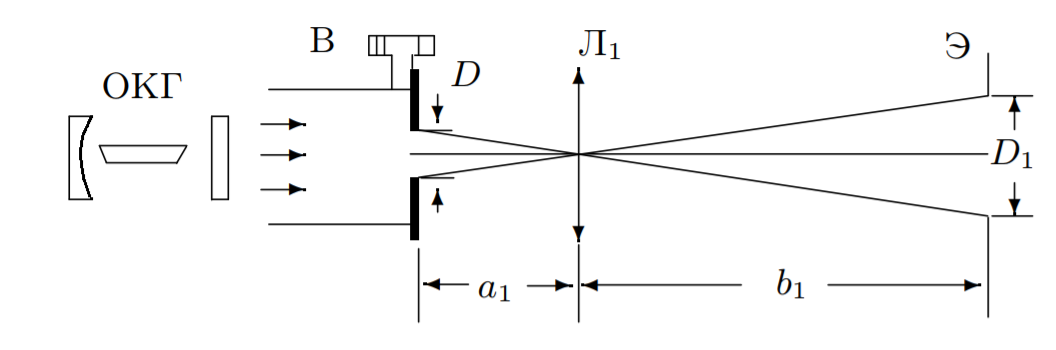
\includegraphics[width = 12 cm]{1.png}
	\caption{Схема для определения ширины щели с помощью линзы}
\end{figure}
 1) Собрали схему и с помощью линзы с $F_1$=43mm получили увеличенное изображение щели(начало отсчета - 13 делений, одно деление - 10 мкм). \\
 
 2) Меняя ширину щели от 5 до 50 делений от нового нуля,
сняли зависимость размера изображения D1 от ширины щели D. Результаты занесли в таблицу:\\
\begin{center}

\begin{tabular}{|c|c|}
\hline 
D, mkm & $D_1$, mm \\ 
\hline 
100 & 2.4 \\ 
\hline 
170 & 3.9 \\ 
\hline 
220 & 5.1 \\ 
\hline 
270 & 6.8 \\ 
\hline 
320 & 7.1 \\ 
\hline 
420 & 11\\ 
\hline 
500 & 12.7 \\ 
\hline 
\end{tabular} 
 \end{center}

 3) Экспериментально измерили a1=165 mm, b1=1165 mm, L=a1+b1=1330 mm\\
 4) Зная L и $F_1$ найдем a1 и b1 по формуле линзы: $\frac{1}{F_1}=\frac{1}{a1}+\frac{1}{b1}$\\
 a1=45 mm, b1=1285 mm $\Rightarrow$ Г=$\frac{b1}{a1}=\frac{D_1}{D_l}=28$\\
	
	 \begin{tabular}{|c|c|c|c|c|c|c|}
 \hline 
 \text{Изображение}, $m*10^{-3}$ & $2.4$ & $3.9$ & $5.1$ & $7.1$ & $11$ & $12.7$ \\ 
 \hline 
 $D_l$, $m*10^{-4}$ & $0.86$ & $1.4$ & $1.82$ & $2.54$ & $3.93	$ & $4.54$ \\ 
 \hline 
  $\text{D}$, $m*10^{-4}$ & $1$ & $1.7$ & $2.2$ & $3.2$ & $4.2$ & $5$ \\ 
 \hline 
 \end{tabular} 
 \\
 
	

\textbf{Определение ширины щели по её спектру}
\begin{figure}[H]
	\centering
	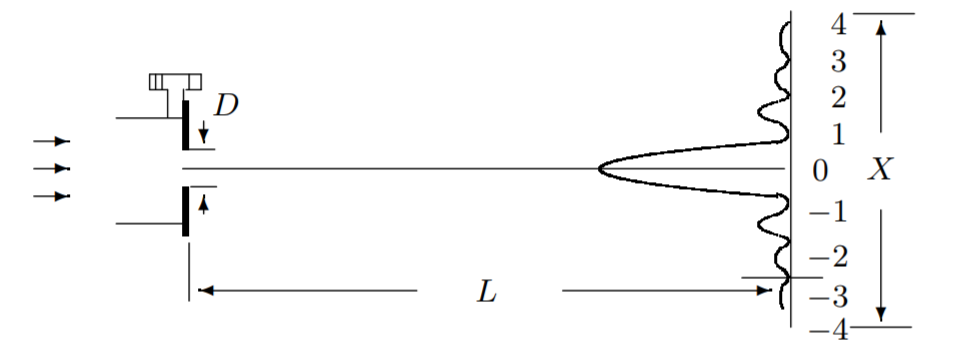
\includegraphics[width = 12 cm]{2.png}
	\caption{Схема для определения ширины щели по спектру}
\end{figure}
 5) Получили на удалённом экране спектр щели. Меняя ширину
щели. Оценили интервал, для которого можно наблюдать и измерять спектр: 23-53 деления.\\
 6) Измерили ширину спектра для самой маленькой щели(100 мкм): 85 mm.\\

 7) Провели серию измерений X(m), меняя ширину щели. Результаты занесли в таблицу:\\
 
\begin{center}
\begin{tabular}{|c|c|c|c|c|c|c|c|c|c|c|c|}
\hline 
 \multicolumn{2}{c|}{10, del} & \multicolumn{2}{c|}{17, del} & \multicolumn{2}{c|}{27, del}  & \multicolumn{2}{c|}{32, del} & \multicolumn{2}{c|}{40, del} & \multicolumn{2}{c|}{50, del} \\ 
\hline 
m & X, mm & m & X, mm  & m & X, mm  & m & X, mm  & m & X, mm  & m & X, mm  \\ 
\hline 
1 & 15 & 1 & 10 & 1 & 5 & 1 & 5 & 1 & 4 & 1 & 3 \\ 
\hline 
2 & 30 & 2 & 15 & 2 & 10 & 2 & 10 & 2 & 8 & 2 & 6 \\ 
\hline 
3 & 45 & 3 & 25 & 3 & 15 & 3 & 15 & 3 & 12 & 3 & 9 \\ 
\hline 
4 & 60 & 4 & 35 & 4 & 20 & 4 & 20 & 4 & 16 & 4 & 12 \\ 
\hline 
\end{tabular} 
\end{center}

 8)Используя соотношение: $D_c=\frac{\lambda * L *2m	}{X}$, рассчитаем ширину щели( $\lambda = 6328 A$, L=1315 mm)\\
 \begin{center}
 
 \begin{tabular}{|c|c|c|c|c|c|c|}
 \hline 
 \text{D}, $m*10^{-4}$ & $1$ & $1.7$ & $2.7$ & $3.2$ & $4$ & $5$ \\ 
 \hline 
 $D_c$, $m*10^{-4}$ & $1.11$ & $1.93$ & $3.32$ & $3.32$ & $4.16$ & $5.55$ \\ 
 \hline 
 \end{tabular} 
  \end{center}

 
  9) Построим графики $D_l(D), D_c(D)$:\\
 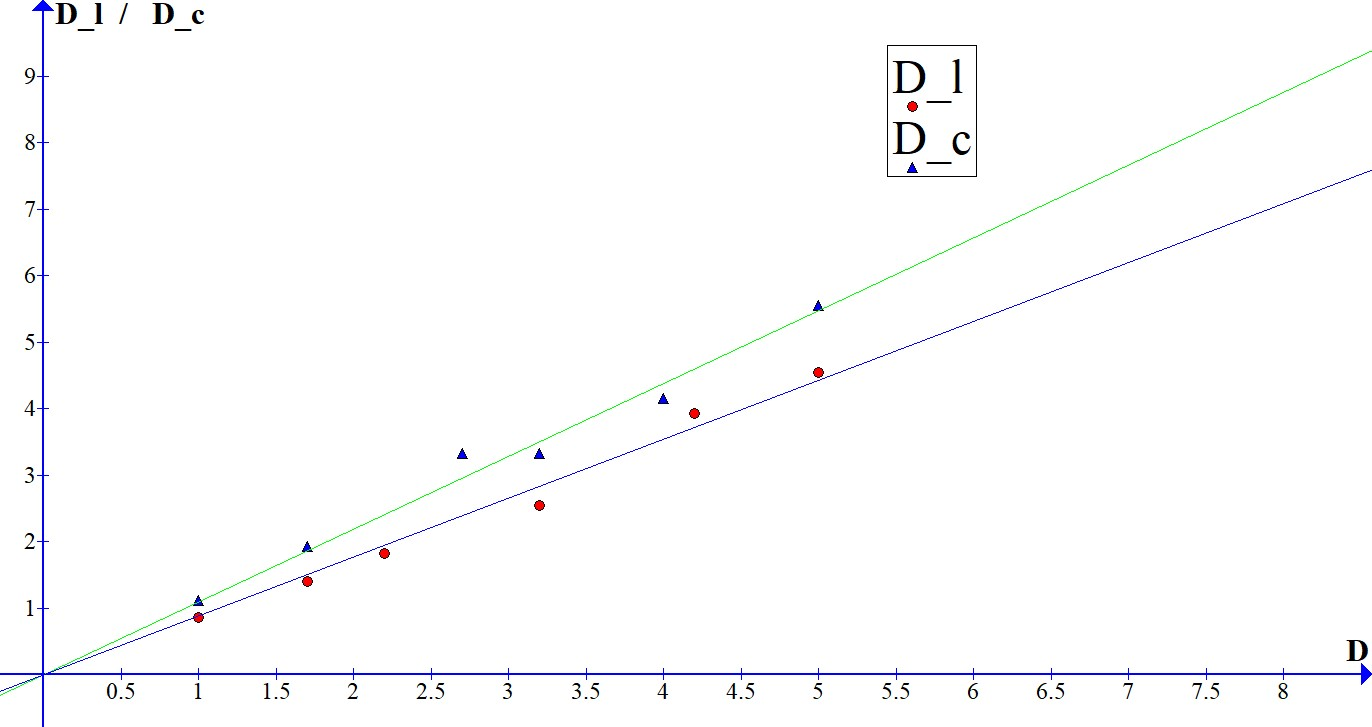
\includegraphics[scale=0.34]{4341}

\textbf{Определение периода решеток}
Определение периода по спектру на удалённом экране\\
\begin{figure}[H]
	\centering
	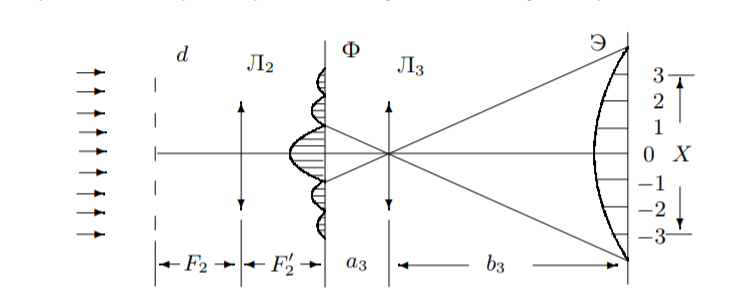
\includegraphics[width = 12 cm]{3.png}
	\caption{Схема для определения ширины щели по спектру}
\end{figure}
 10) Поставили кассету с двумерными решетками вплотную к лазеру.\\
 11) Для каждой сетки измерили расстояние X	между m-ыми максимумами. L=1355 mm\\
 \begin{center}
 

 \begin{tabular}{|c|c|c|c|c|c|c|c|c|c|c|}
 \hline 
 $\text{Сетка:}$ & \multicolumn{2}{c|}{1} & \multicolumn{2}{c|}{2} & \multicolumn{2}{c|}{3} & \multicolumn{2}{c|}{4} &\multicolumn{2}{c|}{5} \\ 
 \hline 
 m & X, mm & $\bigtriangleup X$ & X, mm& $\bigtriangleup X$ & X, mm& $\bigtriangleup X$& X, mm& $\bigtriangleup X$ & X, mm& $\bigtriangleup X$ \\ 
 \hline 
 1 & 4&  17.5 & 2& 12.5  & 2 & 6.25& 2 & 3.75& 2 &2.5\\ 
 \hline 
 2 & 70 && 50& & 25& & 15& & 10& \\ 
 \hline 
 3 & 105&  & 100 && 50& & 25& & 20& \\ 
 \hline 
 4 & 140&  & 150& & 75& & 40& & 30& \\ 
 \hline 
 \end{tabular} 
 
\end{center}
12) Используя формулу  $d_c=\frac{\lambda * L *2m	}{X}$ найдем $d_c$: \\
\begin{center}


 \begin{tabular}{|c|c|c|c|c|c|}
 \hline 
 \text{N сетки} & $1$ & $2$ & $3$ & $4$ & $5$  \\ 
 \hline 
 $d_c$, $m*10^{-5}$ & $5$ & $6.7$ & $13$ & $23$ & $33$  \\ 
 \hline 
 \end{tabular} 
  \end{center}

\textbf{Определение периода решёток по увеличенному изображению спектра}
\begin{figure}[H]
	\centering
	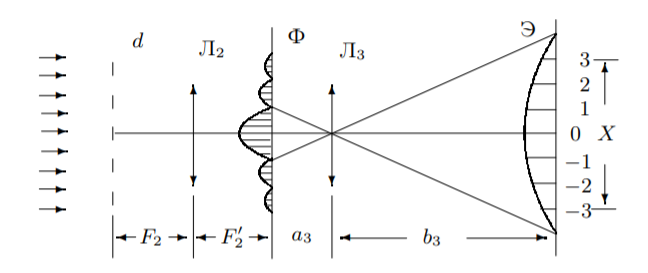
\includegraphics[width = 12 cm]{4.png}
	\caption{Схема определения периода решётки по увеличенному
изображению спектра}
\end{figure}
13) Измерим X и m для всех сеток, где это возможно: \\
\begin{center}

\begin{tabular}{|c|c|c|c|}
\hline 
 \text{N сетки} & 3 & 4 & 5 \\ 
\hline 
m & X, mm & X, mm & X, mm \\ 
\hline 
1 & 6 & 8 & 15 \\ 
\hline 
2 & 12 & 35 & 45 \\ 
\hline 
3 & 28 & 55 & 75 \\ 
\hline 
\end{tabular} 
\end{center}

	14) Зная, что Г3=b3/a3=1.5, F2=11 cm, найдем период сетки по формуле  $d_l=\frac{\lambda *F_2* \text{Г3} *2m	}{X}$       \
	\begin{center}
	
	\begin{tabular}{|c|c|c|c|}
	\hline  
	N & 3 & 4 & 5 \\ 
	\hline 
	$d_l, mm$ & 0.02 & 0.011 & 0.008 \\ 
	\hline 
	\end{tabular} 
	
	\textbf{Мультиплицирование}
	
	\begin{figure}[H]
	\centering
	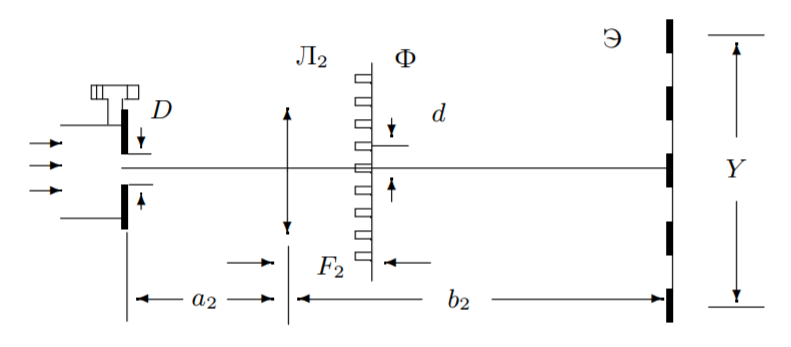
\includegraphics[width = 12 cm]{5.png}
	\caption{Схема для наблюдения мультиплицирования}
\end{figure}
\end{center}
15) Снова поставили тубус со щелью
к окну лазера 
и нашли на
экране резкое изображение щели с помощью линзы
Л2 (F2 = 11 см).
В фокальной плоскости
Ф линзы
Л2 поставили
кассету с сетками.\\
	16) Подобрали такую ширину входной щели
D, чтобы на экране можно было
наблюдать мультиплицированное изображение для всех сеток($a_2=220mm, b_2=1060mm$).\\
	17)Сняли зависимость
Y 
и
K (число промежутков между изображениями) от
№ (номер
сетки) для фиксированной ширины входной щели. Результаты занесли в таблицу: \\
\begin{center}

\begin{tabular}{|c|c|c|c|c|c|c|c|c|}
\hline 
N, сетки & \multicolumn{2}{c|}{1} & \multicolumn{2}{c|}{2} & \multicolumn{2}{c|}{3} &\multicolumn{2}{c|}{4} \\ 
\hline 
Y, mm & 50 & 100 & 35 & 60 & 15 & 30 & 12 & 16 \\ 
\hline 
K & 15 & 40 & 10 & 20 & 8 & 16 & 4 & 8 \\ 
\hline 
\end{tabular} 
	\end{center}

	
	18) Используя формулы $\bigtriangleup y=\bigtriangleup Y/Г2, \bigtriangleup Y=Y/K$ получим:\\
	\begin{center}
	
	\begin{tabular}{|c|c|c|c|c|c|}
	\hline 
	N & 1 & 2 & 3 & 4 & 5 \\ 
	\hline 
	$\bigtriangleup y$, mm & 0.69 & 0.73 & 0.39 & 0.52 & 1 \\ 
	\hline 
	$1/d_c 10^3$ ,1/m & 20 & 15 & 7.7 & 4.34 & 3.03\\
	\hline
	\end{tabular} 
		\end{center}
		И построим график $\bigtriangleup y$($1/d_c$):\\
		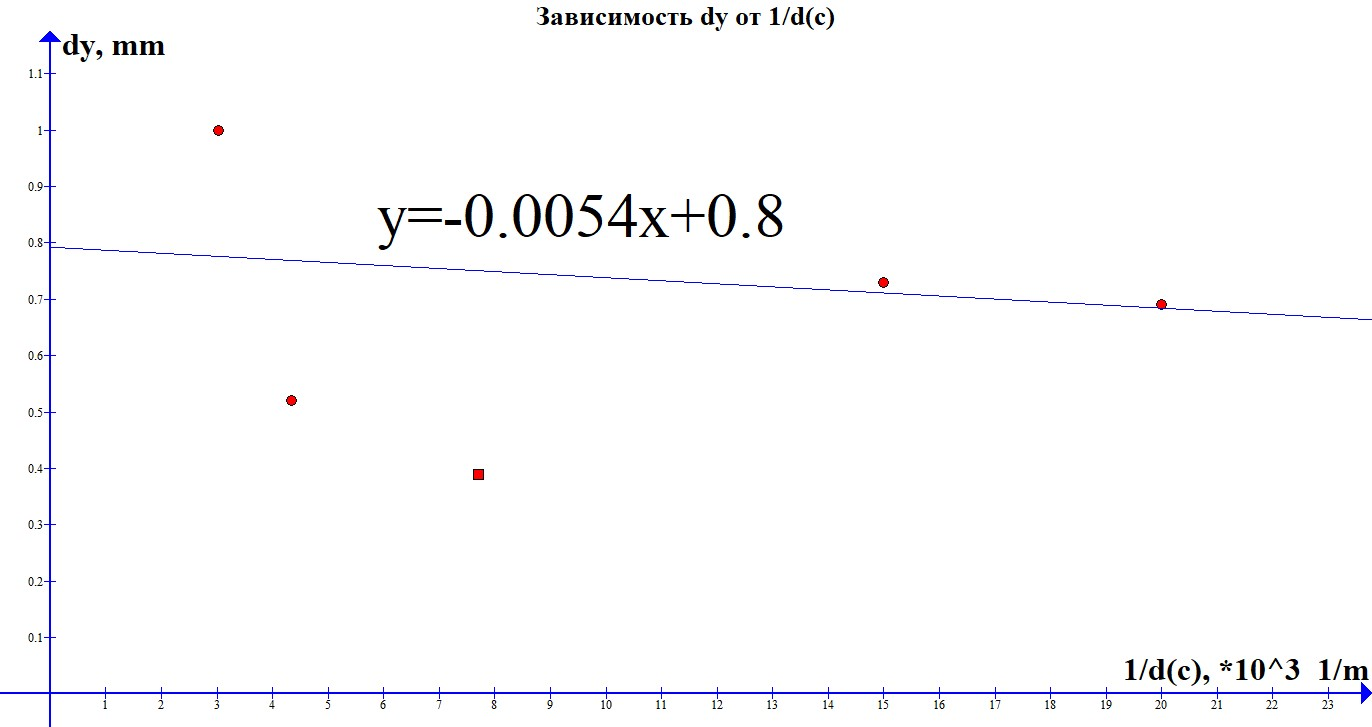
\includegraphics[scale=0.33]{4342}

	
	
	
	
	
	
	
	
	
	
	
	
	
	
	






































\end{document} % конец документа
